\documentclass{article}

\usepackage{amsmath}
\usepackage{amssymb}
\usepackage{booktabs}
\usepackage{hyperref}
\usepackage[utf8]{inputenc}
\usepackage[a4paper, margin=2cm]{geometry}
\usepackage{graphicx}
\usepackage{wrapfig}
\usepackage{float}
\usepackage[spanish]{babel}

\newcommand{\partder}[1]{\frac{\partial}{\partial 1}

\title{Cálculo de la región de decisión}
\author{Pedro Gómez Martín}

\begin{document}
\maketitle

\section{Introducción}
En la teoría de detección, para la decisión óptima en función de la
potencia media $(P_e)$ debemos de dividir el un plano cartesiano en
regiones de decisión para determinar la señal transmitida teniendo
en cuenta la distorsión y atenuación que produce la transmisión.

Para realizar las divisiones debemos tener en cuenta la probabilidad
de cada una de las señales, en este caso consideraremos señales
equiprobables.

\section{Intuición}
Asumiendo que no hay dos señales representadas en el mismo punto del
plano cartesiano y que conforme aumentamos la distancia al punto que
se obtiene colocando el vector que representa una señal en el origen
la probabilidad de que esa fuera la señal transmitida decrece, podemos
asignar a cada punto del plano un valor proporcional a dicha
probabilidad.

\begin{align}
  \label{eq:intuition}
  f_n(x,y) = \frac{1}{\left( x - x_n \right)^2 + \left( y - y_n \right)^2  }
\end{align}

\begin{figure}[H]
  \centering
  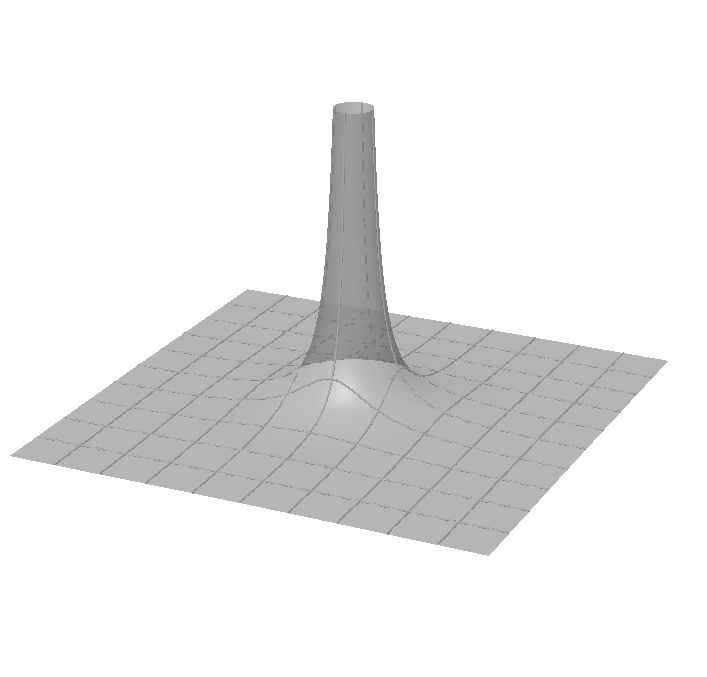
\includegraphics[width=7cm]{./media/potencial_punto.png}
  \caption{Grafica potencial un punto}
  \label{fig:potential1}
\end{figure}

\section{Desarrollo}
Pensando en la función $f_n(x,y)$\ref{eq:intuition} como una función de
potencial, podemos desarrollar el campo vectorial asociado a ella y
mediante el principio de superposición podemos obtener el campo que
dicta la tendencia a la señal transmitida.

\begin{align}
  \label{eq:development}
  F_n = -\nabla f_n\left( x, y \right) &= -\nabla \frac{1}{\left( x - x_n \right)^2 + \left( y - y_n \right)^2}\\
  &= \partdev{x}
\end{align}

\end{document}